%This is the homework 2 latex file for problem 1

\documentclass[12pt]{article}
\usepackage{amsfonts}
\usepackage{amssymb}
\usepackage{graphicx}
\usepackage{mathtools}
\usepackage{color}
\usepackage{fancyhdr}
\usepackage[margin=2cm]{geometry}
\DeclarePairedDelimiter\ceil{\lceil}{\rceil}
\DeclarePairedDelimiter\floor{\lfloor}{\rfloor}
\pagestyle{fancy}


\begin{document}
\fancyhfoffset[L]{0cm}
\fancyhfoffset[R]{0cm}
\chead{Tyler Ayrton Stank}

%\begin{centering}
%Tyler Ayrton Stank
%\end{centering}

\begin{enumerate}
    \setcounter{enumi}{0}
    %1
    \item
    \begin{enumerate}
        %1a
        \item
        \begin{enumerate}
            %1ai
            \item
            $i_1$:
                $$z = (-1\times0) + (-3.5\times1) + (1\times1.5) = 0 -3.5 + 1.5 = -2$$
                $$g(z) = \frac{1}{1 + e^{-(-2)}} = 0.1192$$
            $i_2$:
                $$z = (2.5\times0) + (2\times1) + (1\times-0.5) = 0 + 2 - 0.5 = 1.5$$
                $$g(z) = \frac{1}{1+e^{-1.5}} = 0.8176$$
            $o$:
                $$z = (-1.5\times0.1192) + (2.5\times0.8176) + (1\times0.5) = 2.3651$$
                $$g(z) = 0.9141$$
            %1aii
            \item
                $i_1$:\\
                Prediction: $g(z) = 0.9141$\\
                Desired output: $g^*(z) = 1.0000$\\
                Error: 0.0859\\
                $\Delta w_{i,j} = \alpha a_i a_j (1-a_j) \sum w_{j,k} (T_k - O_k) O_k (1-O_k)$\\
                $\Delta w_{x_1,i_1} = 0.1 \times 0 \times 0.1192 \times (1-0.1192) \times \sum w_{i_1,o} (1.0 - 0.9141) 0.9141 (1-0.9141)$\\
                $ = 0 \times \sum w_{i_1,o} \times 0.006745$\\
                $ = 0$\\
                $\Delta w_{x_2,i_1} = 0.1 \times 1 \times 0.1192 \times (1-0.1192) \times \sum w_{i_1,o} \times (0.006745)$\\
                $ = 0.1050 \times 0.006745 \times \sum w_{i_1,o}$\\
                $ = 0.0007082 \times 1.5 = 0.001062$\\
                $\Delta w_{j,k} = \alpha a_j (T_k - O_k) O_k (1-O_k)$\\
                $\Delta w_{i_1,o} = 0.1 \times 0.1192 \times 0.006745 = 0.00008040$\\
                \\
                $w_{x_1, i_1} = w_{x_1,i_1} + \Delta w_{x_1,i_1} = 2.5 + 0 = 2.5$\\
                $w_{x_2, i_1} = w_{x_2,i_1} + \Delta w_{x_2,i_1} = 2 + 0.001062 = 2.001062$\\
                $w_{i_1, o} = w_{i_1,o} + \Delta w_{i_1,o} = -1.5 + 0.00008040 = -1.4999196$\\
                \\
                $i_2$:\\
                Prediction: $g(z) = 0.9141$\\
                Desired output: $g^*(z) = 1.0000$\\
                Drror: 0.0859\\
                $\Delta w_{i,j} = \alpha a_i a_j (1-a_j) \sum w_{j,k} (T_k - O_k) O_k (1-O_k)$\\
                $\Delta w_{x_1,i_2} = 0.1 \times 0 \times 0.8176 \times 0.1824 \times \sum w_{i_2,o} \times 0.006745$\\
                $ = 0 \times \sum w_{i_2,o} \times 0.006745 = 0$
                $\Delta w_{x_2,i_2} = 0.1 \times 1 \times 0.8176 \times 0.1824 \times \sum w_{i_2,o} \times 0.006745$\\
                $ = 0.01491 \times 0.006745 \times \sum w_{i_2,o} = 0.0001006 \times 2.5 = 0.0002515$\\
                $\Delta w_{j,k} = \alpha a_j (T_k - O_k) O_k (1-O_k)$\\
                $\Delta w_{i_2,o} = 0.1 \times 0.8176 \times 0.006745 = 0.0005515$\\
                \\
                $w_{x_1, i_1} = w_{x_1,i_2} + \Delta w_{x_1,i_2} = -1 + 0 = -1$\\
                $w_{x_2, i_1} = w_{x_2,i_2} + \Delta w_{x_2,i_2} = -3.5 + 0.0002515 = -3.4997485$\\
                $w_{i_2, o} = w_{i_2,o} + \Delta w_{i_2,o} = 2.5 + 0.0005515 = 2.5005515$\\
        \end{enumerate}

        %1b
        \item 
            \textcolor{white}{.}\vspace{-12pt}\\
            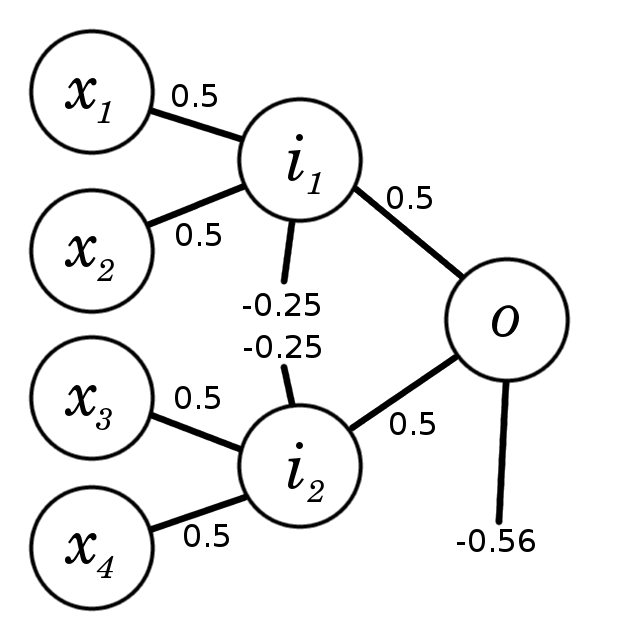
\includegraphics[width=8cm]{P1b}

    \end{enumerate}
\end{enumerate}

\end{document}


